\chapter{Resultados}

\label{chap:result}
Os resultados obtidos nos desafios foram:
%--------- NEW SECTION ----------------------
\section{Webots}

Cada um dos 16 sensores de distância incluídos no Pionner são encontrados no arquivo de controle do robô challengecontroller.c
e contêm valores de peso para cada roda, que são baseados na posição do sensor no robô e mostram como sua leitura influencia o 
comportamento do duas rodas. Além disso, o valor do peso auxilia na tomada de decisão, pois, se a leitura de algum sensor cair 
abaixo do valor mínimo definido, significa que o robô está próximo a um obstáculo e deve mudar de direção usando um dos casos acima. 
No final, ele foi usado para determinar o comportamento do robô em todos os valores de peso em cada roda vezes um fator de velocidade, 
que é dependente tanto da relação de leitura do sensor quanto do valor de distância mínima.

Também faz parte do controle o sensor de luz que foi adicionado para completar o desafio, 
este sensor ativa o estado STOP quando detecta um brilho maior que 750 W / m2 e assim o desafio é concluído.

As fotos mostram o pioneer iniciando, chegando na área luminosa e parando no tempo correto, completando assim o desafio proposto,
para uma melhor visualização da solução tem um link do video logo abaixo e o controle pode ser encontrado no repositório https://github.com/marcellabecker/desafiorobotica 

\begin{figure} [h!]	
    \centering
    \caption{Pioneer iniciando o percurso}
    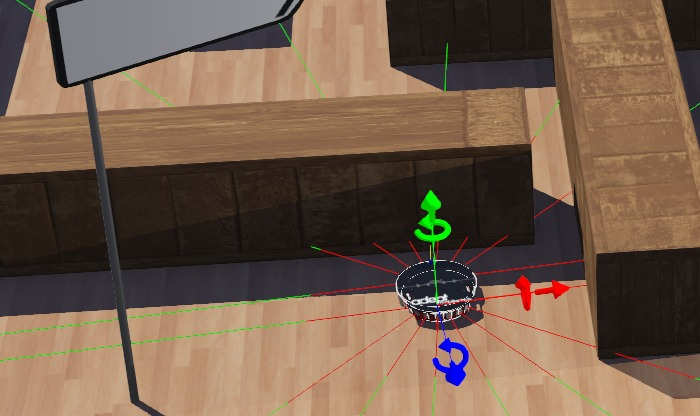
\includegraphics[width=0.5\textwidth]{inicio.jpeg}
    \caption*{Fonte:Própria.}
    \label{fig:inciodopercurso}
\end{figure}

\begin{figure} [h!]	
    \centering
    \caption{Pioneer completando o percurso}
    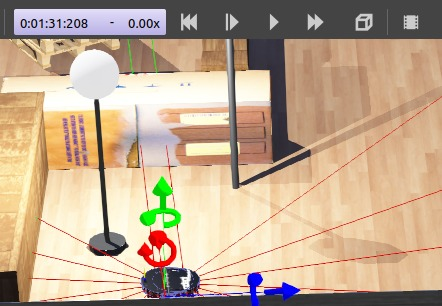
\includegraphics[width=0.5\textwidth]{fim.jpeg}
    \caption*{Fonte:Própria.}
    \label{fig:fimdopercurso}
\end{figure}



Link para assistir ao vídeo:https://www.youtube.com/watch?v=RftRevxZUOE

\section{Turtlesim SETPOINT}
Inicialmente no codigo foi feita uma função de callback que é chamada quando o subscriber recebe um dado do tópico. 
Logo depois o nó é iniciado, para que possa ser feito os publishers e subscribers no tópicos, sendo assim 
vel-publisher publica mensagens no tópico cmd-vel e posecb recebe a msg de coodenada da posição.

Goal-x e goal-y recebem os inputs das coordenadas x e y para onde a tartaruga deve ir. 

kp-lin e kp-ang são os controles de velocidade linear e angular definidos para que a tartaruga nao ande muito rapido nem
muito devagar e controla o seu angulo de curvatura durante o movimento.

A FUNÇÃO is-shutdown() verifica se seu programa deve sair, portanto enquanto não entrar no if que está dentro do while significa que o erro ainda é 
maior que 0.1 e a turtle ainda não chegou ao seu destino sendo assim o programa deve continuar rodando, ate que o o erro seja 0.1 como manda o desafio
e ela deve parar.

As figuras abaixos mostram a janela da turtle antes da coordenadas e depois dela andar para coordenada (1,1).

\begin{figure} [h!]	
    \centering
    \caption{janela da turtle}
    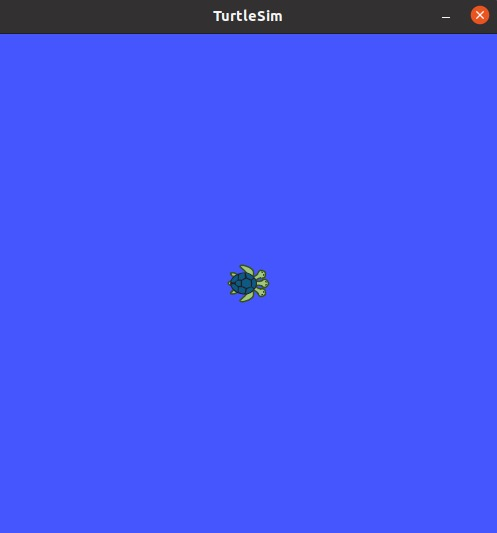
\includegraphics[width=0.35\textwidth]{antes.jpeg}
    \caption*{Fonte:Própria.}
    \label{fig:inicio}
\end{figure}

\begin{figure} [h!]	
    \centering
    \caption{Turtle chegou ao destino}
    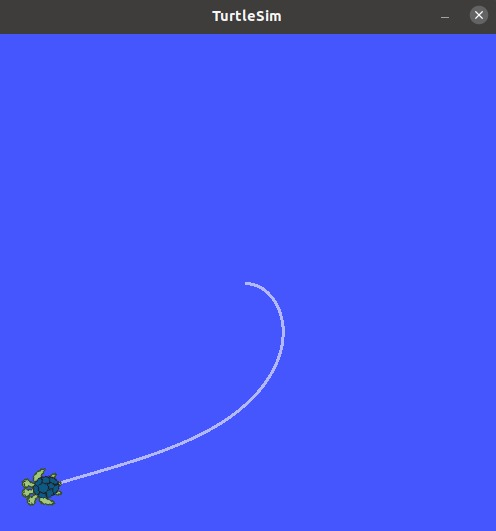
\includegraphics[width=0.35\textwidth]{depois.jpeg}
    \caption*{Fonte:Própria.}
    \label{fig:fim}
\end{figure}
Para uma melhor visualização da solução tem um link do video 
logo abaixo e o controle pode ser encontrado no repositório https://github.com/marcellabecker/turtle  

Link para assistir ao vídeo:https://youtu.be/NNkwSgDScuY
\section{Husky}
\subsection{Move-base}
Com todos os comando de movimentação já configurados e as janelas rviz e gazebo ja abertas a movimentação é feita pelo mouse podendo também usar o teclado pelo comando teleop-twist-keyboard ou por controle remoto.
As imagens abaixo mostram antes, durante e depois que a movimentação for concluida. 

\begin{figure} [h!]	
    \centering
    \caption{Husky antes do movimento}
    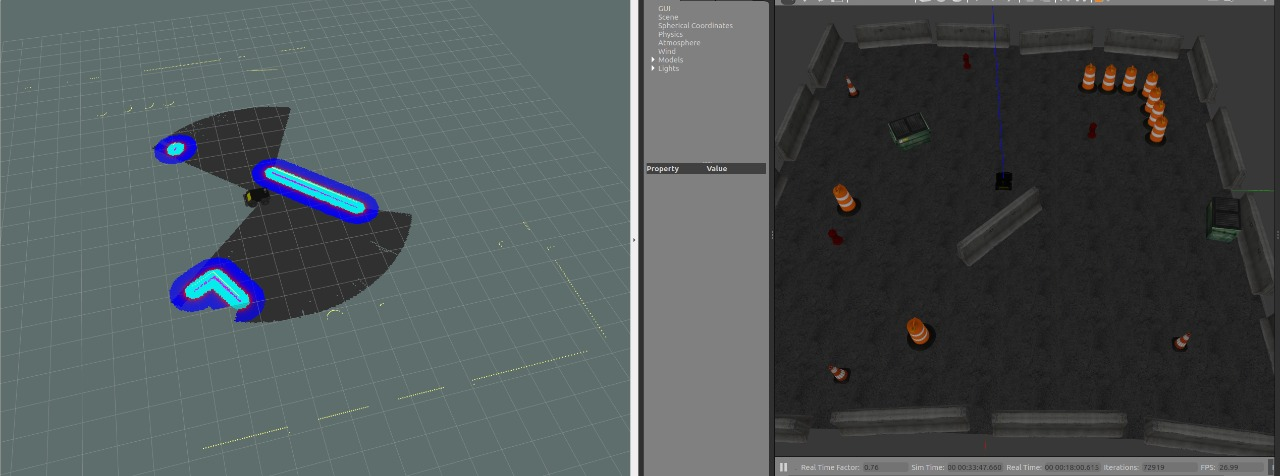
\includegraphics[width=0.7\textwidth]{antesmb.jpeg}
    \caption*{Fonte:Própria.}
    \label{fig:antesmovebase}
\end{figure}
\begin{figure} [h!]	
    \centering
    \caption{Husky durante o movimento}
    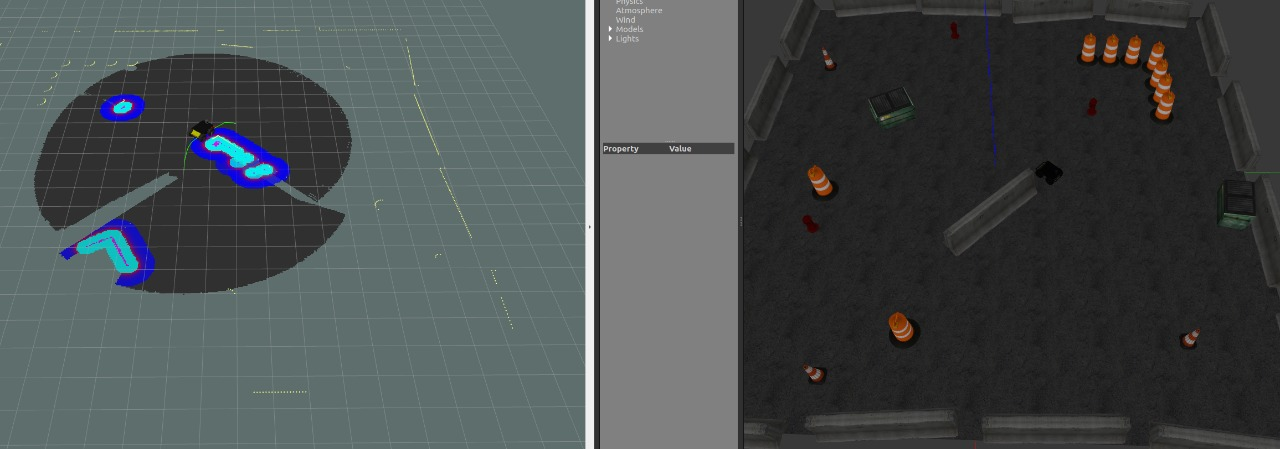
\includegraphics[width=0.7\textwidth]{durantemb.jpeg}
    \caption*{Fonte:Própria.}
    \label{fig:durantemovebase}
\end{figure}
\begin{figure} [h!]	
    \centering
    \caption{Husky depois o movimento}
    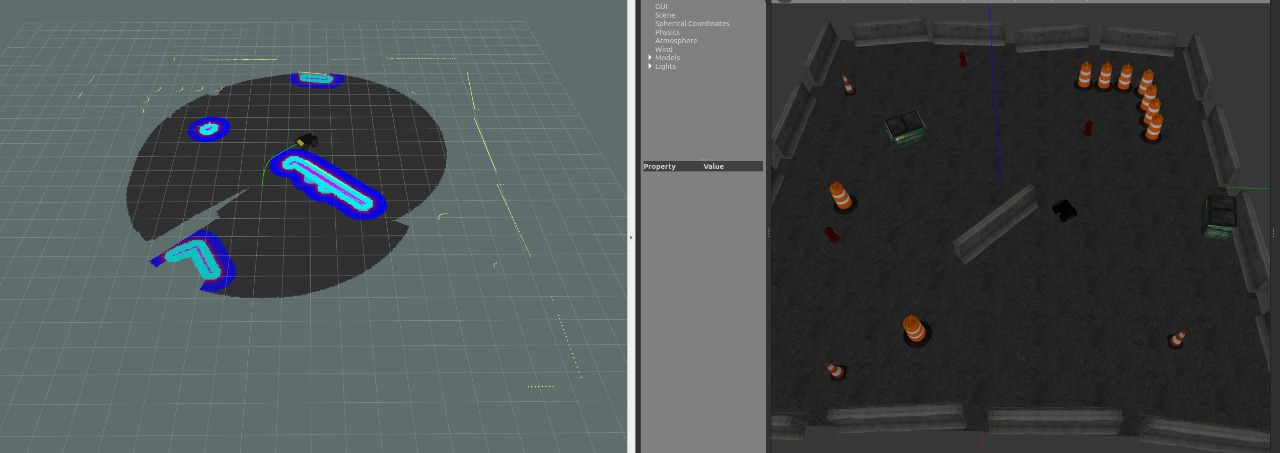
\includegraphics[width=0.7\textwidth]{depoismb.jpeg}
    \caption*{Fonte:Própria.}
    \label{fig:depoismovebase}
\end{figure}
\subsection{AMCL}
Com todos os comando de movimentação já configurados e as janelas rviz e gazebo ja abertas a movimentação é feita pelo mouse podendo também usar o teclado pelo comando teleop-twist-keyboard ou por controle remoto.
As imagens abaixo mostram antes, durante e depois que a movimentação for concluida.
\begin{figure} [h!]	
    \centering
    \caption{Husky antes do movimento}
    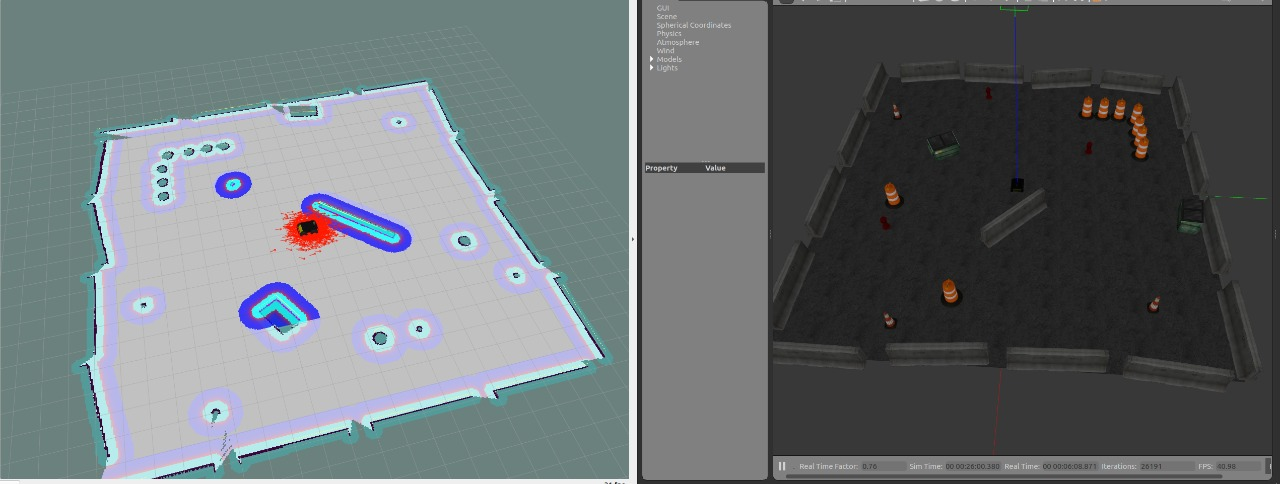
\includegraphics[width=0.7\textwidth]{antesamcl.jpeg}
    \caption*{Fonte:Própria.}
    \label{fig:antesamcl}
\end{figure}
\begin{figure} [h!]	
    \centering
    \caption{Husky durante o movimento}
    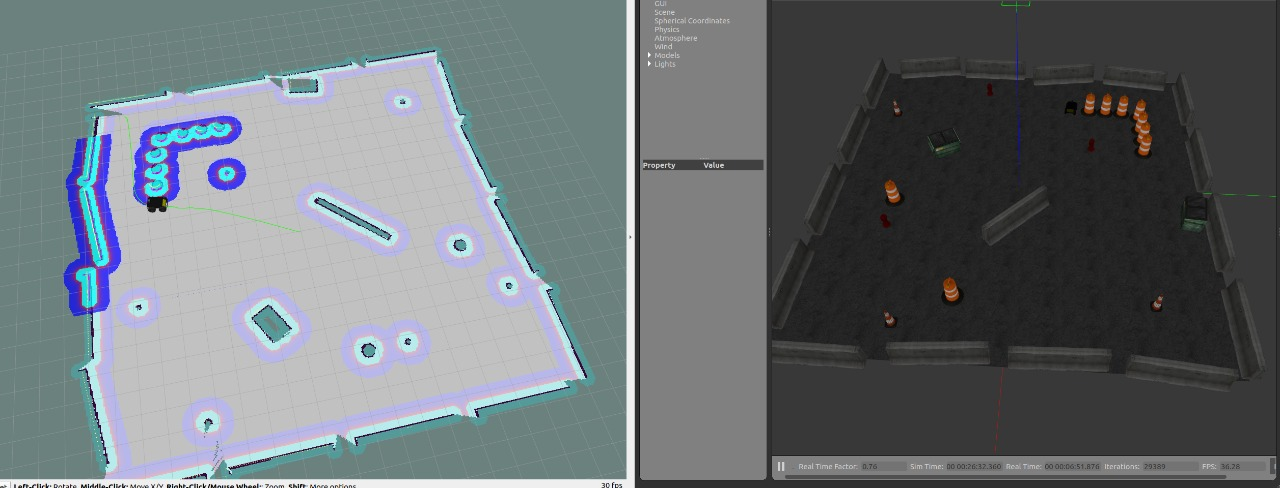
\includegraphics[width=0.7\textwidth]{duranteamcl.jpeg}
    \caption*{Fonte:Própria.}
    \label{fig:duranteamcl}
\end{figure}
\begin{figure} [h!]	
    \centering
    \caption{Husky depois o movimento}
    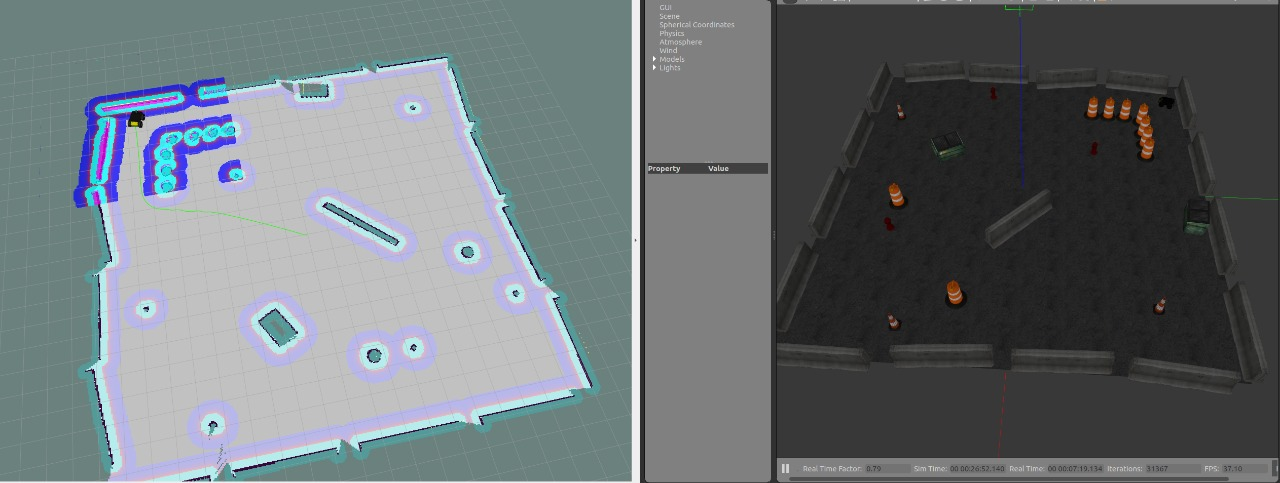
\includegraphics[width=0.7\textwidth]{depoisamcl.jpeg}
    \caption*{Fonte:Própria.}
    \label{fig:depoisamcl}
\end{figure}
É possivel ver que diferente do move-base o Husky consegue ter um alcance bem maior de visualização, o todos formados pelo mapa e o laiser destaca os que estão mais perto.
\subsection{Gmapping}
Com todos os comando de movimentação já configurados e as janelas rviz e gazebo ja abertas a movimentação é feita pelo mouse podendo também usar o teclado pelo comando teleop-twist-keyboard ou por controle remoto.

As imagens abaixo mostram antes, durante e depois que a movimentação for concluida.
\begin{figure} [h!]	
    \centering
    \caption{Husky antes do movimento}
    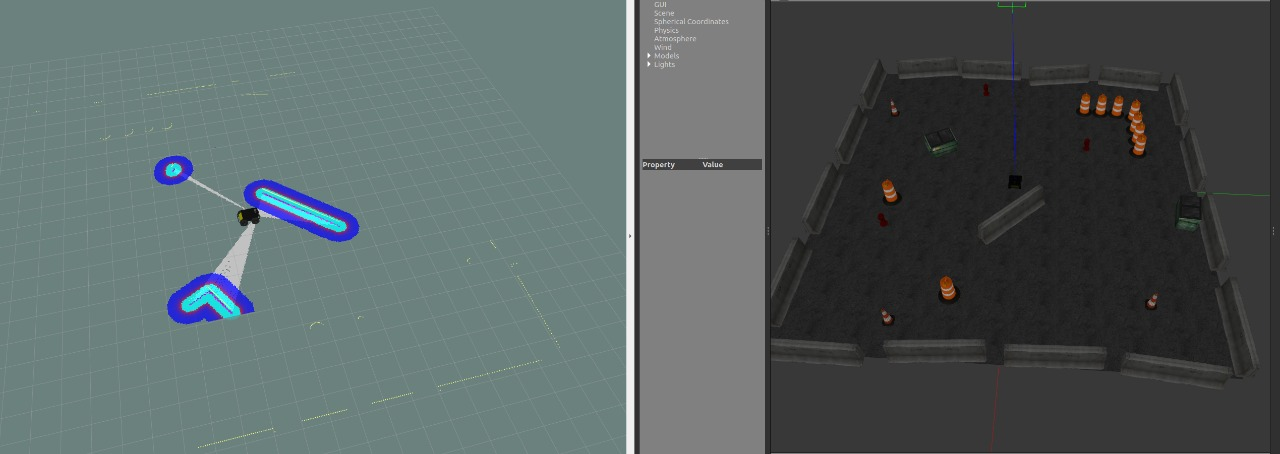
\includegraphics[width=0.7\textwidth]{antesgm.jpeg}
    \caption*{Fonte:Própria.}
    \label{fig:antesgmappinng}
\end{figure}
\begin{figure} [h!]	
    \centering
    \caption{Husky durante o movimento}
    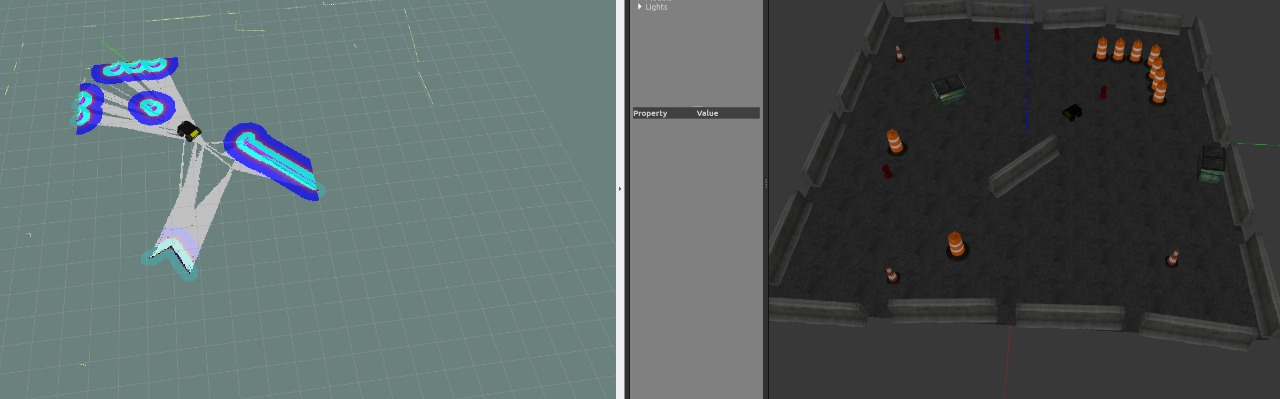
\includegraphics[width=0.7\textwidth]{durantegm.jpeg}
    \caption*{Fonte:Própria.}
    \label{fig:durantegmapping}
\end{figure}
\begin{figure} [h!]	
    \centering
    \caption{Husky depois o movimento}
    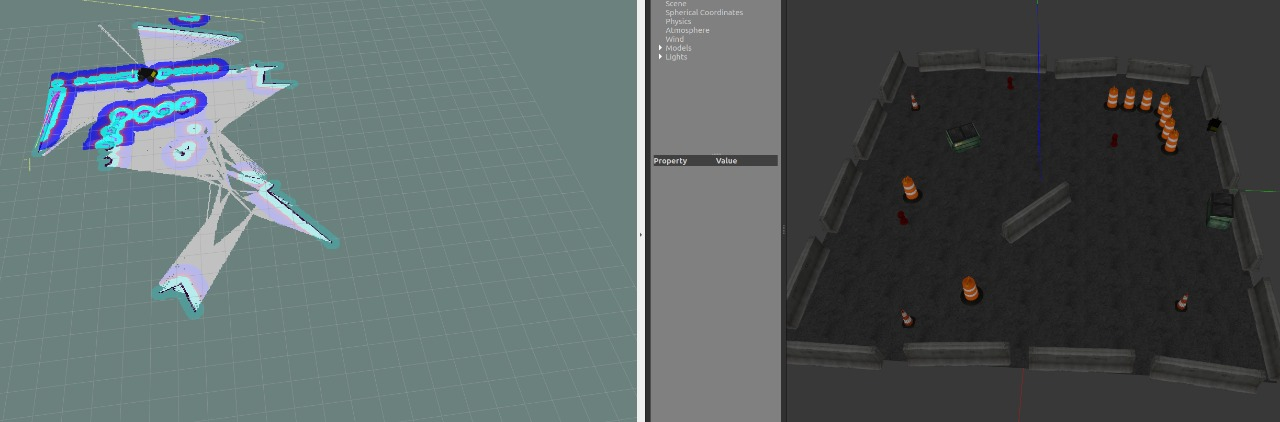
\includegraphics[width=0.7\textwidth]{depoisgm.jpeg}
    \caption*{Fonte:Própria.}
    \label{fig:depoisgmapping}
\end{figure}



A diferença do Gmapping é o SLAM que localiza e mapeia o ambiente simultâneamente, como pode ser visto o Husky enquando está se localizando para andar no mapa, também constrói o mapa.
\subsection{Frontier-exploration}
Com todos os comando de movimentação já configurados e as janelas rviz e gazebo ja abertas a movimentação é feita pelo mouse podendo também usar o teclado pelo comando teleop-twist-keyboard ou por controle remoto.

As imagens abaixo mostram antes, durante e depois que a movimentação for concluida.
\begin{figure} [h!]	
    \centering
    \caption{Husky antes do movimento}
    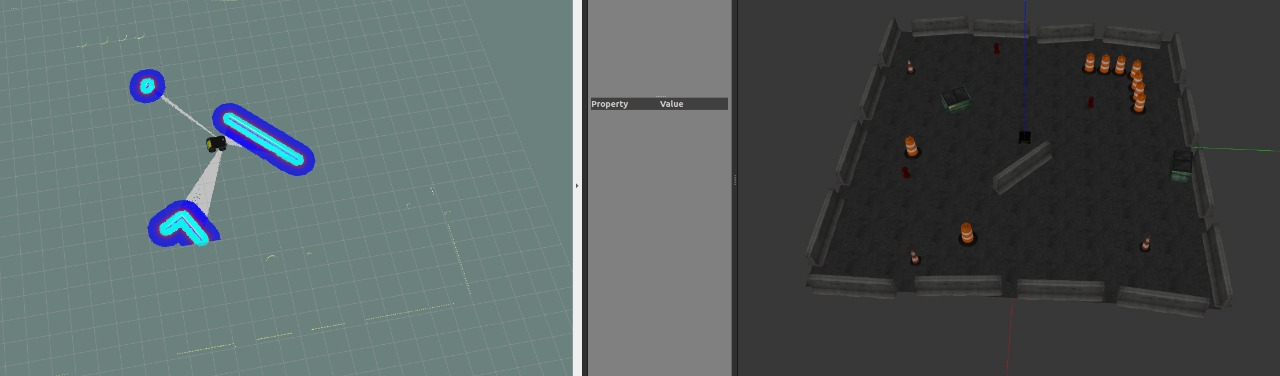
\includegraphics[width=0.7\textwidth]{antesf.jpeg}
    \caption*{Fonte:Própria.}
    \label{fig:antesFrontier-exploration}
\end{figure}
\begin{figure} [h!]	
    \centering
    \caption{Husky durante o movimento}
    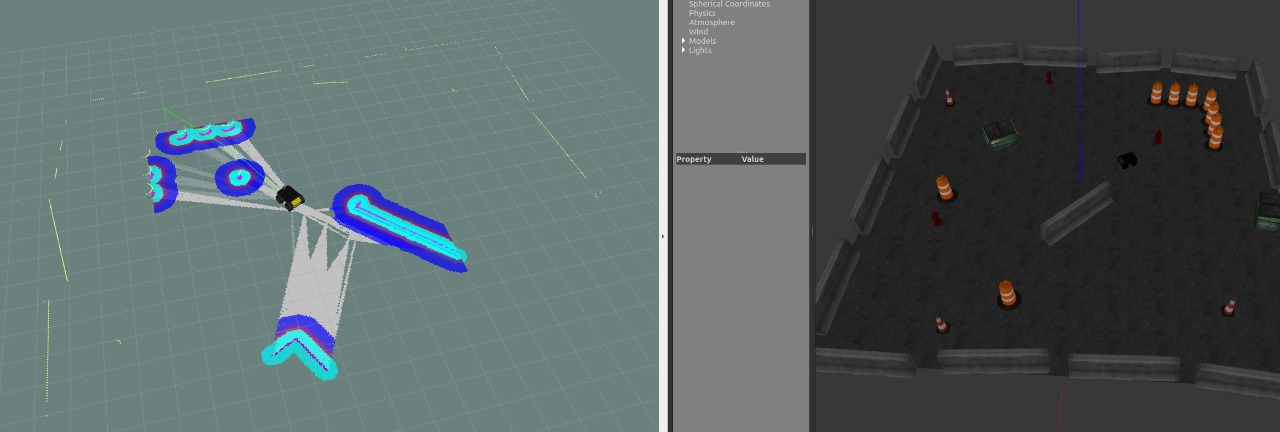
\includegraphics[width=0.7\textwidth]{durantef.jpeg}
    \caption*{Fonte:Própria.}
    \label{fig:duranteFrontier-exploration}
\end{figure}
\begin{figure} [h!]	
    \centering
    \caption{Husky depois o movimento}
    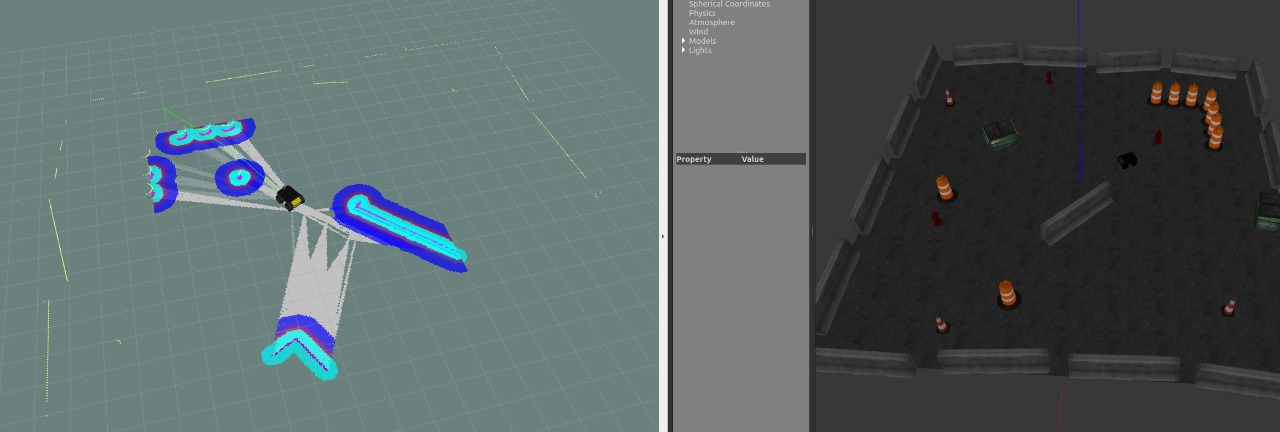
\includegraphics[width=0.7\textwidth]{depoisf.jpeg}
    \caption*{Fonte:Própria.}
    \label{fig:depoisFrontier-exploration}
\end{figure}

Conforme o robô se move, você deve ver o mapa estático cinza crescer. Ocasionalmente, o algoritmo de gmapping irá realocar o robô, causando um salto discreto no mapa. Quando a meta de exploração for concluída, você verá uma mensagem escrito DONE na janela do terminal.
\section{cpp}
-Desafio do Triângulo de Pascal:
Para demonstrar os resultados obtidos foi compilado o codigo, a figura a baixo mostra o resultado da linha 4 do triangulo.
\begin{figure} [h!]	
    \centering
    \caption{triangulo ate linha 4}
    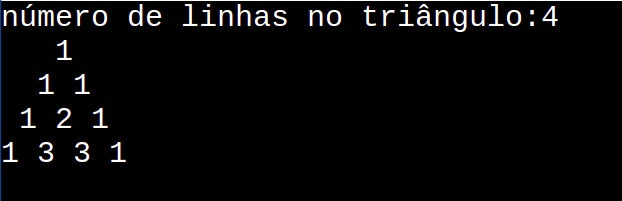
\includegraphics[width=0.5\textwidth]{rt.jpeg}
    \caption*{Fonte:Própria.}
    \label{fig:triangulodepascal}
\end{figure}

- Permutação de cordas:
Após o codigo ser bildado foi colocado a palavra tia como no exemplo do PDF dado, na figura a baixo mostra o resultado.
\begin{figure} [h!]	
    \centering
    \caption{Permutação da palavra tia}
    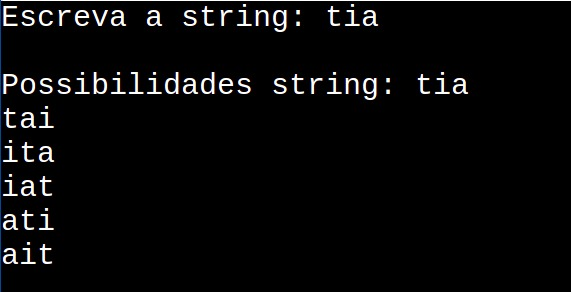
\includegraphics[width=0.3\textwidth]{rp.jpeg}
    \caption*{Fonte:Própria.}
    \label{fig:permutacao}
\end{figure}
- Autoimpressão:
%\begin{figure} [h!]	
%    \centering
%    \caption{Permutação da palavra tia}
%    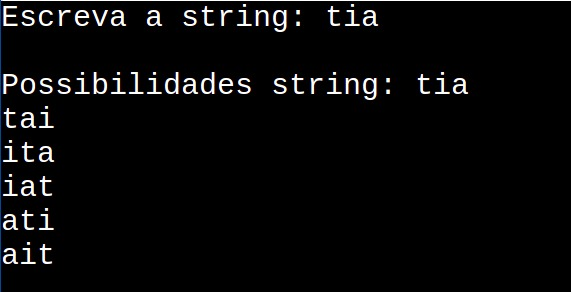
\includegraphics[width=0.7\textwidth]{rp.jpeg}
%    \caption*{Fonte:Própria.}
%    \label{fig:permutacao}
%\end{figure}

\section{Python 1}
-Mediana de Três Valores:
Após colocar os 3 números foi o programa cálculou a médiada dos 3 através da formula.

Como pode ser visto na figura abaixo:
\begin{figure} [h!]	
    \centering
    \caption{Mediana}
    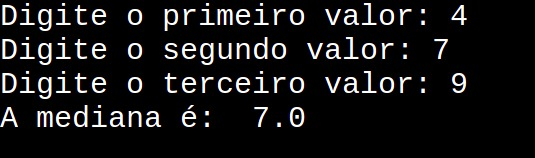
\includegraphics[width=0.3\textwidth]{mediana1.jpeg}
    \caption*{Fonte:Própria.}
    \label{fig:med}
\end{figure}

-Os Doze Dias do Natal:
Nesse desafio foi feita a plotagem completa da musica The twelve Days of christmas.

O resultado pode ser visualizado na imagem:
\begin{figure} [h!]	
    \centering
    \caption{Musica}
    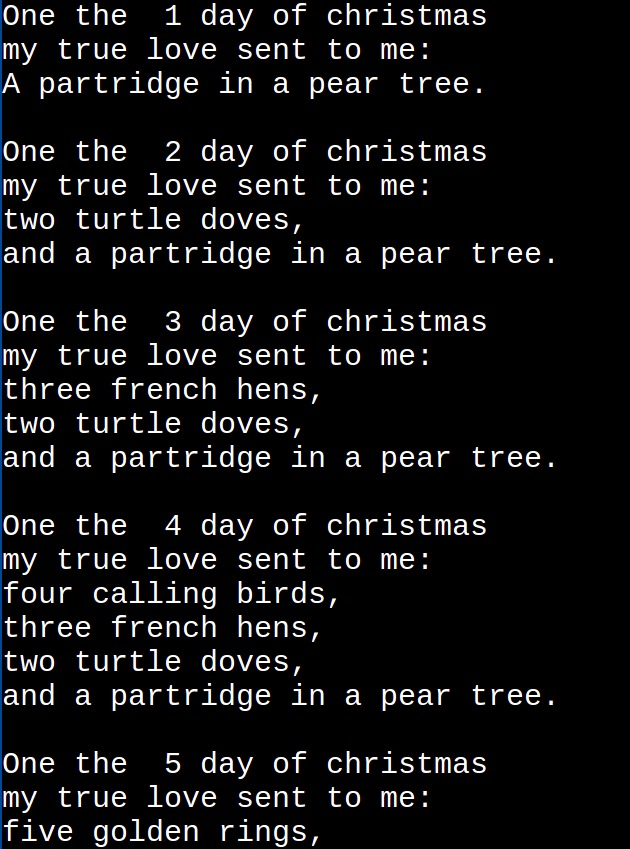
\includegraphics[width=0.3\textwidth]{12.jpeg}
    \caption*{Fonte:Própria.}
    \label{fig:musica}
\end{figure}

-Centralize uma corda no terminal:

Nesse desafio aṕos a escolha da palavra centralização e dos espados de 25 foi plotada de forma certralizada ao terminal de 25 espaços vazios.
O resultado pode ser visualizado na imagem:
\begin{figure} [h!]	
    \centering
    \caption{centralização}
    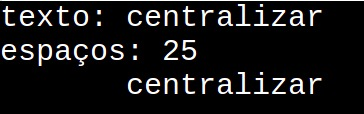
\includegraphics[width=0.3\textwidth]{central.jpeg}
    \caption*{Fonte:Própria.}
    \label{fig:centralizar}
\end{figure}

-Capitalize-o:

Nesse desafio foi posto uma frase começando com letra minuscula e um nome após os ; também minusculos e foi corrigido.
O resultado pode ser visualizado na imagem:
\begin{figure} [h!]	
    \centering
    \caption{Maiúsculo e minúsculo}
    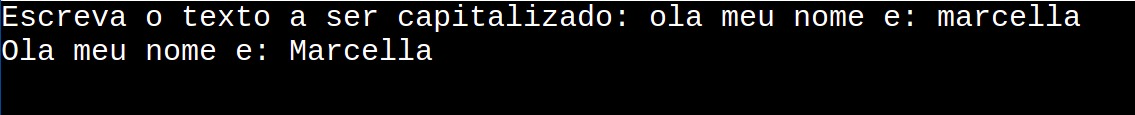
\includegraphics[width=0.5\textwidth]{cap.jpeg}
    \caption*{Fonte:Própria.}
    \label{fig:cap}
\end{figure}

-Uma string representa um inteiro:

\begin{figure} [h!]	
    \centering
    \caption{Não inteiro}
    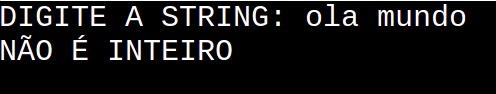
\includegraphics[width=0.3\textwidth]{stg.jpeg}
    \caption*{Fonte:Própria.}
    \label{fig:stg}
\end{figure}

-É um número primo?
Nesse Desafio será mostrado se o numero é primo ou não.

\begin{figure} [h!]	
    \centering
    \caption{primo}
    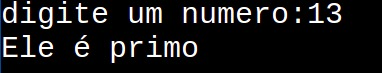
\includegraphics[width=0.3\textwidth]{primo.jpeg}
    \caption*{Fonte:Própria.}
    \label{fig:primo}
\end{figure}

-Senha aleatória:
Faz uma senha aleatória de 7 a 10 caracteres usando a tabela ASCII
resultado pode ser visto a baixo:
\begin{figure} [h!]	
    \centering
    \caption{senha aleatória}
    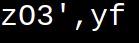
\includegraphics[width=0.3\textwidth]{alea.jpeg}
    \caption*{Fonte:Própria.}
    \label{fig:senhaaleatoria}
\end{figure}

-Verifique uma senha:
Para verificar que a senha está valida a função testa e printa se é ou não valida.
\begin{figure} [h!]	
    \centering
    \caption{senha fraca}
    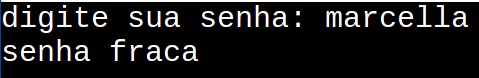
\includegraphics[width=0.3\textwidth]{senhafraca.jpeg}
    \caption*{Fonte:Própria.}
    \label{fig:senhafraca}
\end{figure}
\begin{figure} [h!]	
    \centering
    \caption{senha ok}
    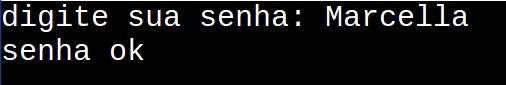
\includegraphics[width=0.3\textwidth]{senhaok.jpeg}
    \caption*{Fonte:Própria.}
    \label{fig:senhaok}
\end{figure}

-Conversões de base arbitrária:
Nesse desafio é convertido os número de uma base para outra escolhida como mostrado abaixo:

\begin{figure} [h!]	
    \centering
    \caption{Número convertido}
    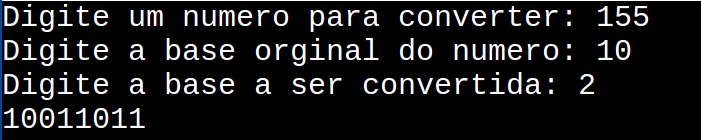
\includegraphics[width=0.3\textwidth]{convert.jpeg}
    \caption*{Fonte:Própria.}
    \label{fig:convert}
\end{figure}

-Reduzir uma fração aos termos mais baixos:
Simplifica frações para a menor possivel como mostra a seguir:
\begin{figure} [h!]	
    \centering
    \caption{frações}
    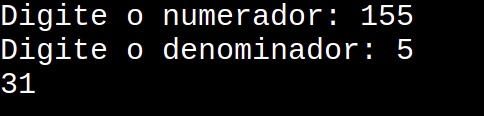
\includegraphics[width=0.3\textwidth]{fracoes.jpeg}
    \caption*{Fonte:Própria.}
    \label{fig:fracao}
\end{figure}

-Reduzir Medidas:
Faz a manipulação das medidas para quantidade digitada.
Logo a seguir tem um exemplo:

\begin{figure} [h!]	
    \centering
    \caption{Medidas}
    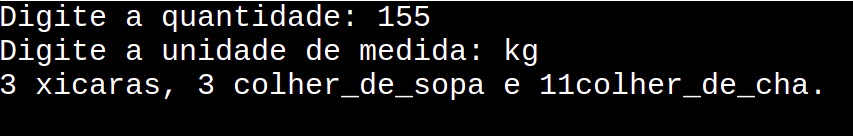
\includegraphics[width=0.3\textwidth]{medidas.jpeg}
    \caption*{Fonte:Própria.}
    \label{fig:medidas}
\end{figure}

-Datas mágicas:
Mostra todas a datas mágicas de 1900 ate 2000:

\begin{figure} [h!]	
    \centering
    \caption{Data mágica}
    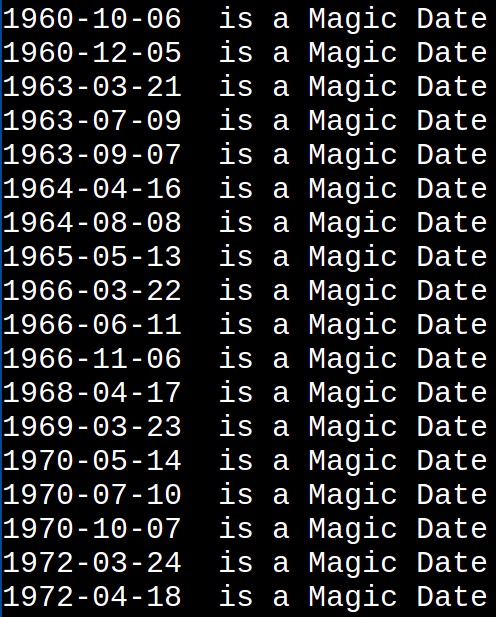
\includegraphics[width=0.3\textwidth]{datam.jpeg}
    \caption*{Fonte:Própria.}
    \label{fig:datamagica}
\end{figure}

\section{Python 2}

-Cifra de César:
Faz a criptografia de mensagens a seguir um exemplo:

\begin{figure} [h!]	
    \centering
    \caption{Crifitografia}
    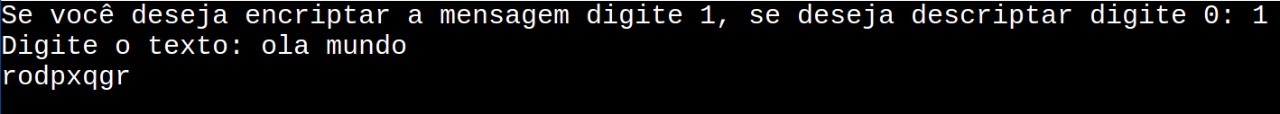
\includegraphics[width=0.3\textwidth]{crip.jpeg}
    \caption*{Fonte:Própria.}
    \label{fig:criptografia}
\end{figure}

-Verifique uma senha:
Este é muito parecido com um do primeiro workbook e mostra se a senha é valida ou não.

\begin{figure} [h!]	
    \centering
    \caption{Digite outra senha}
    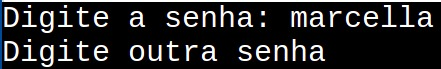
\includegraphics[width=0.3\textwidth]{senha.jpeg}
    \caption*{Fonte:Própria.}
    \label{fig:Senha}
\end{figure}

-Números perfeitos:
Mostra os números perfeitos de 1 até 10000

\begin{figure} [h!]	
    \centering
    \caption{Números perfeitos}
    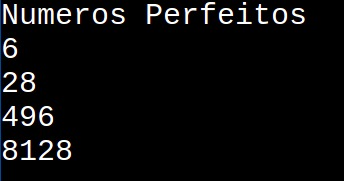
\includegraphics[width=0.3\textwidth]{perfeito.jpeg}
    \caption*{Fonte:Própria.}
    \label{fig:Numerosperfeitos}
\end{figure}

-Palíndromo Recursivo:
Mostra se a palavra digitada é ou não um palindromo.
\begin{figure} [h!]	
    \centering
    \caption{Palindromos}
    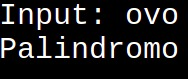
\includegraphics[width=0.3\textwidth]{palindromo.jpeg}
    \caption*{Fonte:Própria.}
    \label{fig:palindromo}
\end{figure}